
\chapter{UMLDesigner}
\label{chap:UMLDesigner}


UMLDesigner is a graphical tooling to edit and visualize UML models created by the French company: \textit{Obeo}.

It is an open source software.

\begin{figure}[h]
  \centering
  
\includegraphics[width=0.3\textwidth]{logo}
  \caption{UMLDesigner logo}
  \label{fig:logo}
\end{figure}

\section{Kernel}

UMLDesigner is based on a Eclipse kernel. The interface is the same as Eclipse. You can notice on figure \ref{fig:umldesigner} that the menu are the same in the both software.

UMLDesigner use also Sirius. Is an Eclipse plugin which permit to represent diagrams. Sirius was created by \textit{Obeo} to Thales.

Then \textit{Obeo} develop a plugin to adapt diagram product by Sirius as UML diagrams.

\begin{figure}[h]
  \centering
  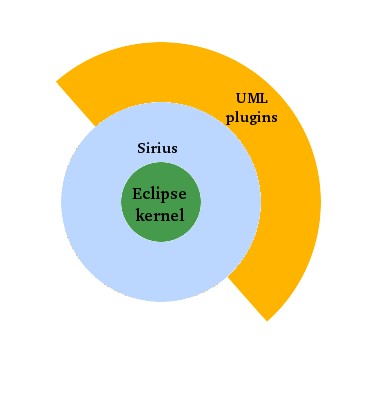
\includegraphics[width=0.5\textwidth]{archi}
  \caption{The UMLDesigner kernel}
  \label{fig:kernel}
\end{figure}

\newpage
\section{Operation}



\begin{figure}[h]
  \centering
  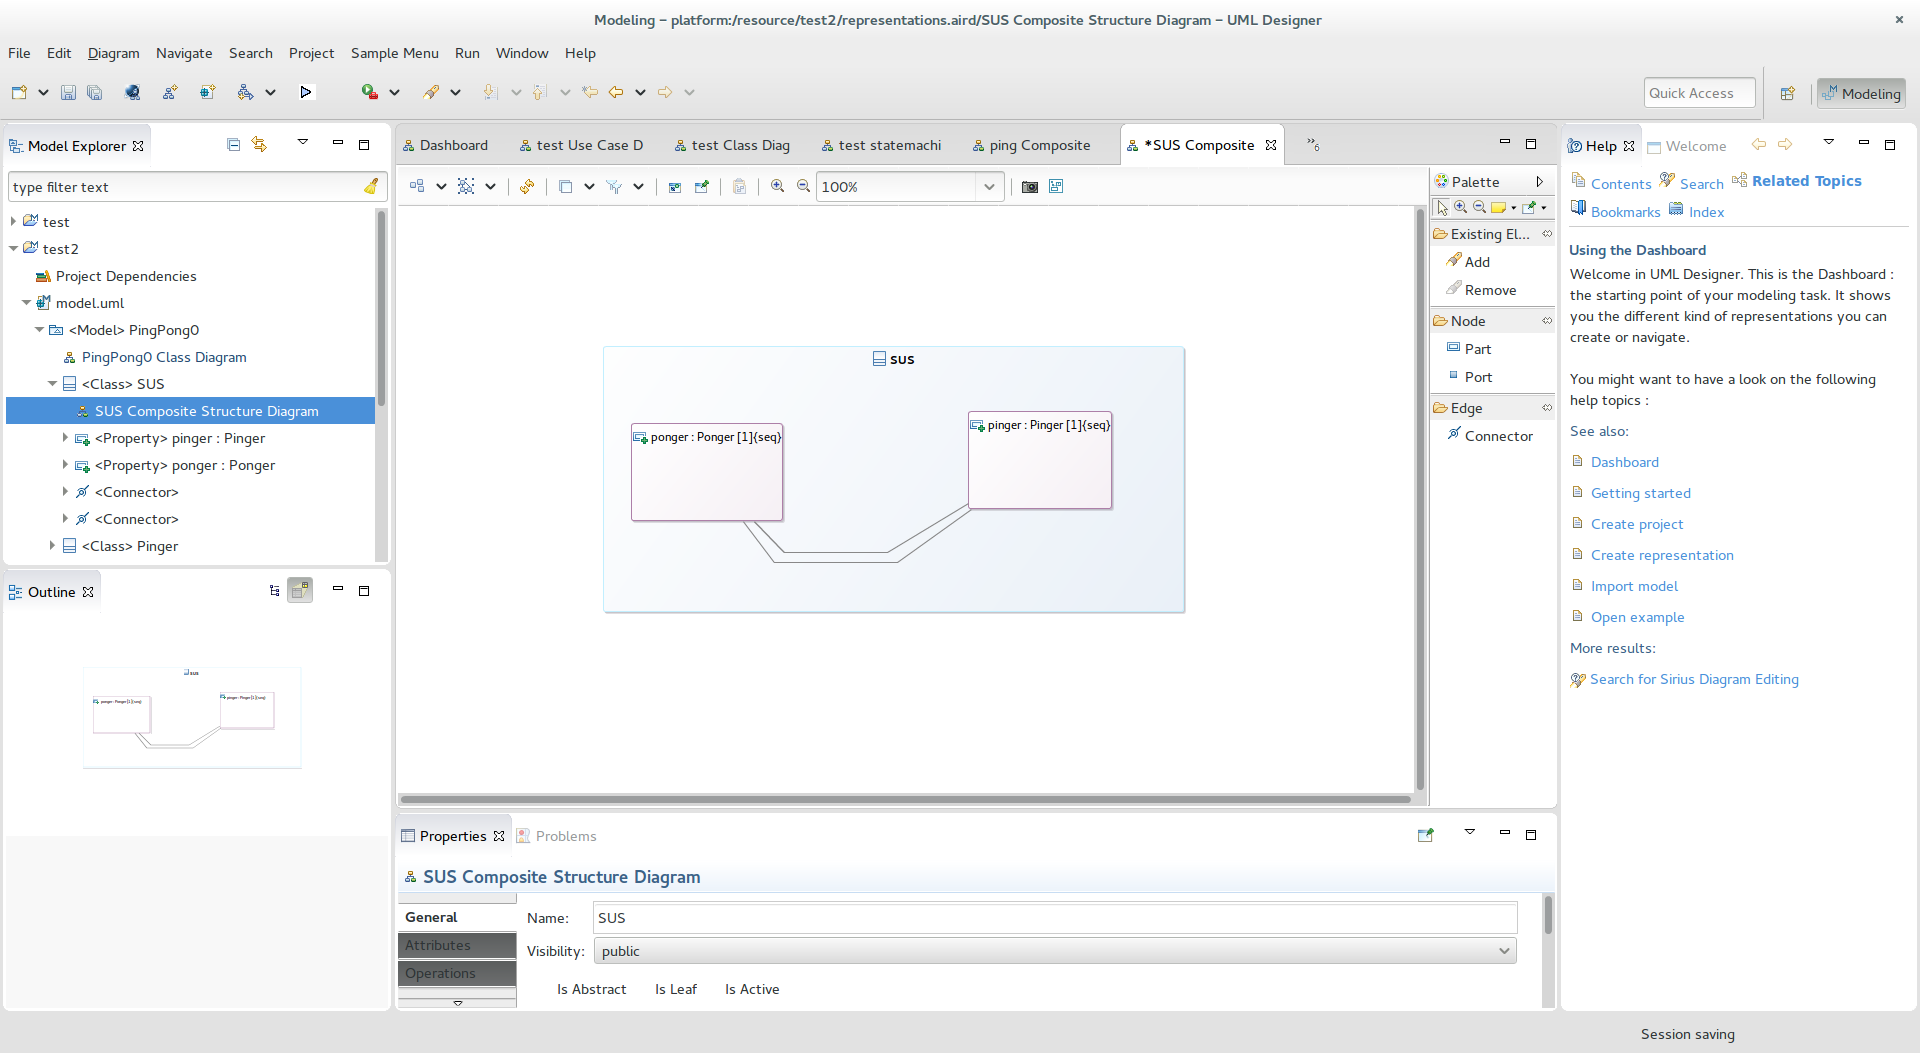
\includegraphics[width=0.8\textwidth]{umldesigner}
  \caption{Screenshot of UMLDesigner}
  \label{fig:umldesigner}
\end{figure}




%%% Local Variables: 
%%% mode: latex
%%% TeX-master: "../rapport_de_base"
%%% End: 
